% !TeX spellcheck = id_ID
\documentclass[a4paper,12pt]{article}
\usepackage[indonesian]{babel}
\usepackage{graphicx}
\usepackage{multirow}
\usepackage{enumitem}
\usepackage{listings}
\usepackage{wrapfig}
\usepackage[T1]{fontenc}
\usepackage{inconsolata}
\usepackage{lipsum}
\usepackage{adjustbox}


\usepackage{color}
\usepackage[table]{xcolor}
\definecolor{mygreen}{rgb}{0,0.6,0}
\definecolor{mygray}{rgb}{0.5,0.5,0.5}
\definecolor{mymauve}{rgb}{0.58,0,0.82}
\lstset{%
    language=java,
    frame=single,                    % Set frame around code
    backgroundcolor=\color{white},   % choose the background color
    basicstyle=\footnotesize,        % size of fonts used for the code
    breaklines=true,                 % automatic line breaking only at whitespace
    captionpos=b,                    % sets the caption-position to bottom
    commentstyle=\color{mygreen},    % comment style
    escapeinside={\%*}{*)},          % if you want to add LaTeX within your code
    keywordstyle=\color{blue},       % keyword style
    stringstyle=\color{mymauve},     % string literal style
}

\graphicspath{ {./img/} }
\begin{document}
\title{ {\Large Laporan Praktikum}\\ Algoritma dan Pemrograman Lanjut\\{\Large Pertemuan 1}}

\author{Aldzikri Dwijayanto Prathama 
	\\195410189
	\\Informatika}
\makeatletter
\begin{titlepage}
	\begin{center}
		{\huge \bfseries \@title }\\[14ex]
		
\includegraphics[scale=.8]{logo}\\[4ex]
		{\large \@author}\\[12ex]
		{\large \bfseries {SEKOLAH TINGGI MANAJEMEN INFORMATIKA DAN KOMPUTER
				AKAKOM YOGYAKARTA}}
	\end{center}


%{\large \@date} 
\end{titlepage}
\makeatother
%\maketitle
\newpage
\tableofcontents
\newpage

\section{Tujuan}
\paragraph{}
Mahasiswa dapat membuat program untuk menyelesaikan kasus menggunakan
perulangan bertingkat 2 maupun 3

\section{Teori}
\paragraph{}
Dalam Java, ada tiga struktur kontrol perulangan yaitu: for, while, dan do-while.
Untuk yang belum tahu: Perulangan ( atau yang disebut Looping) adalah suatu
proses yang diklakukan secara berulang-ulang hingga mencapai kondisi tertentu.
Sebagai contoh ketika anda ingin mencetak deretan angka hingga batas tertentu
(contoh: 1-100), maka anda bisa menggunakan fungsi looping dalam program.
Biasanya fungsi looping digunakan dan berperan penting dalam algoritma
sorting, karena kita akan menukar nilai variabel hingga menghasilkan nilai
berurutan.

\newpage

\section{Pembahasan}
\subsection{Praktik}
\subsubsection{Praktik 1}
\begin{lstlisting}
public class Looping{
    public static void main(String[] args){
        for (int i=1; i<=2;i++ ) {
            for (int j=1;j<=3 ;j++ ) {
            System.out.format("Perulangan [i=%d, j=%d] %n", i,j);
            }
        }
    }
}
\end{lstlisting}
Perulangan di atas akan mengeprint Perulangan [i=x, j=y] ke layar, di mana x diperoleh dari perulangan yang berada di luar, sedangkan y diperoleh dari perulangan yang ada di dalamnya.\\
Sehingga jika dijalankan, maka akan menghasilkan output berikut:\\
\begin{center}
    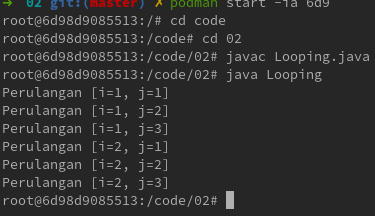
\includegraphics[scale=.7]{1.png}
\end{center}

\begin{lstlisting}
public class Looping{
    public static void main(String[] args){
        for (int i=1; i<=3;i++ ) {
            for (int j=1;j<=2 ;j++ ) {
            System.out.format("Perulangan [i=%d, j=%d] %n", i,j);
            }
        }
    }
}
\end{lstlisting}
Program tersebut sama dengan program sebelumnya, tetapi kondisi pada perulangan diluar dan didalam di tukar, i<=2 menjadi i<=3, sedangkan j<=3 diganti menjadi j<=2.\\
Hasilnya seperti berikut:\\
\begin{center}
    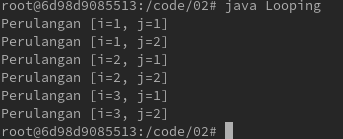
\includegraphics[scale=.7]{2.png}
\end{center}

\subsubsection{Praktik 2}
\begin{lstlisting}
public class Bentuk1
{
    public static void main(String[] args)
    {
        int a = 5;
        for (int b = 1; b <= a; b++)
        {
            System.out.print('*');
            System.out.println();
        }
    }
}
\end{lstlisting}
Program ini memiliki perulangan, yang akan diulang sebanyak 5 kali, yang pernyataannya akan mengeprint bintang, lalu akan mengganti baris. Outputnya seperti berikut:\\
\begin{center}
    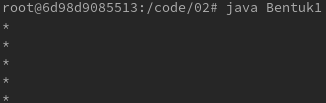
\includegraphics[scale=.7]{3.png}
\end{center}

\newpage

\subsubsection{Praktik 3}
\begin{lstlisting}
public class Bentuk2
{
    public static void main(String[] args) {
        int a = 5;
        for (int b = 1; b <= a; b++){
            for (int c = 1; c <= b; c++) {
                System.out.print('*');
            }
            System.out.println();
        }
    }
}
\end{lstlisting}
Program di atas merupakan program dari praktik 2 yang dimodifikasi dengan menambahkan perulangan di dalam perulangan pertama. Perulangan yang ada didalam akan melakukan perulangan
sejumlah perulangan induknya. Sehinnga program akan menghasilkan output berbentuk segitiga siku-siku seperti berikut:\\
\begin{center}
    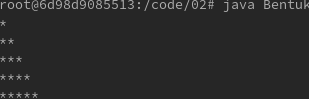
\includegraphics[scale=.7]{4.png}
\end{center}

\newpage
\section{Kesimpulan}

\end{document}
